\chapter{Propuesta de solución}
\label{chap:chapter2}

\section*{Introducción}
\addcontentsline{toc}{section}{Introducción}
Este capítulo presenta la propuesta de solución para abordar el problema identificado en la investigación: la interpretación y contextualización de datos no estructurados del transporte marítimo extraídos del Diario de la Marina (1844–1960). Aquí se detallan los requisitos funcionales (RF) y no funcionales (RNF) que el sistema debe cumplir, así como una descripción exhaustiva de la solución propuesta, incluyendo las historias de usuario y las tarjetas CRC (Clase-Responsabilidad-Colaboración). Además, se analizan los patrones arquitectónicos y de diseño seleccionados para estructurar la aplicación, junto con las buenas prácticas de codificación asociadas a las tecnologías empleadas. Finalmente, se incluyen el diagrama de clases y el diagrama de componentes, que ilustran los elementos clave que integran esta propuesta. Este capítulo sienta las bases técnicas y conceptuales para la implementación y validación descritas en capítulos posteriores, alineándose con los objetivos específicos de diseño e implementación establecidos en la introducción.

\section{Descripción de la Propuesta de Solución}
La solución propuesta consiste en el desarrollo de un sistema multiagente conversacional basado en inteligencia artificial (IA) y procesamiento de lenguaje natural (PLN), diseñado específicamente para transformar datos históricos no estructurados en conocimiento estructurado y accesible. Este sistema se centra en el análisis del transporte marítimo documentado en el Diario de la Marina, abarcando el período de 1844 a 1960, y busca superar las limitaciones identificadas en el estado del arte, como la falta de contextualización histórica y la incapacidad de las herramientas actuales para manejar textos antiguos con precisión. Para ello, integra modelos de lenguaje de gran escala (LLMs), técnicas de Recuperación Aumentada por Generación (RAG), y una arquitectura multiagente que coordina tareas especializadas.
El sistema permite a los usuarios interactuar mediante consultas en lenguaje natural, obteniendo respuestas precisas y contextualizadas que combinan texto y, cuando sea necesario, representaciones gráficas de patrones marítimos (e.g., rutas, cargamentos, frecuencias de puertos). Esta funcionalidad no solo facilita la comprensión de las dinámicas comerciales del Caribe en el período estudiado, sino que también optimiza la investigación histórica al automatizar la extracción y análisis de información. Al hacerlo, contribuye a la preservación del patrimonio documental al hacer accesible un recurso que, de otro modo, permanecería confinado a archivos físicos o datos digitales desorganizados.\\
\begin{figure}[h]
	\centering
	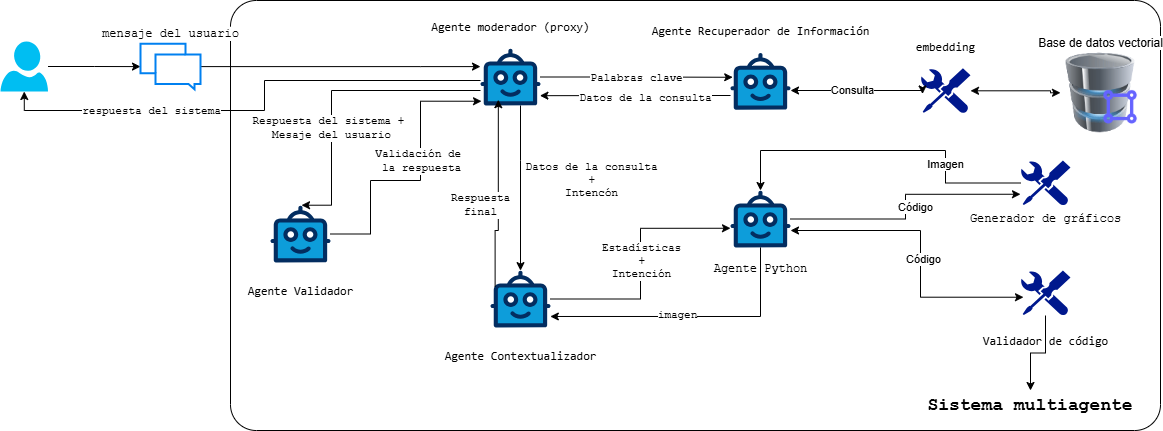
\includegraphics[width=1\textwidth]{images/mas}
	\caption{Esquema general de la propuesta de solución.}
	\label{fig:Propuesta de solución}
\end{figure}\\
La Figura \ref{fig:Propuesta de solución} ilustra el flujo de trabajo del sistema multiagente. El proceso inicia cuando el usuario introduce una consulta en lenguaje natural (e.g., “¿Cuáles fueron los principales puertos de exportación en 1880?”). Esta consulta es recibida por el Agente de Moderación (proxy), que actúa como coordinador central. Este agente extrae palabras clave (e.g., “puertos”, “exportación”, “1880”) y determina la intención del usuario (e.g., consulta informativa o solicitud de análisis estadístico). A continuación, el Agente de Moderación delega la tarea al Agente Recuperador de Información, que convierte las palabras clave en embeddings utilizando un modelo preentrenado y consulta una base de datos vectorial para recuperar fragmentos relevantes del \textit{Diario de la Marina}. Los datos recuperados —como textos sobre actividades portuarias— se devuelven al Agente de Moderación.
Posteriormente, el Agente de Moderación envía la información recuperada, junto con la intención del usuario, al Agente Contextualizador . Este agente evalúa si la consulta requiere una respuesta textual, estadísticas o ambas. Si se necesitan estadísticas (e.g., un gráfico de puertos más activos), genera instrucciones que se envían al Agente Python . Este agente crea un script en Python para procesar los datos y producir visualizaciones (e.g., un gráfico de barras), el cual es validado por una herramienta de análisis de código. Una vez aprobado, una segunda herramienta convierte el script en una imagen gráfica que se retorna al Agente Contextualizador. Si no se requieren gráficos, el Agente Contextualizador enriquece la información con contexto histórico (e.g., eventos económicos relevantes de 1880) utilizando técnicas RAG y datos externos.
Antes de entregar la respuesta al usuario, el Agente Validación revisa la coherencia y precisión del contenido generado, comparándolo con la consulta original para evitar inconsistencias o alucinaciones. Finalmente, el Agente de Moderación ensambla la respuesta validada —que puede incluir texto, imágenes o ambos— y la presenta al usuario en un formato adecuado, completando el ciclo de interacción. Este diseño multiagente asegura una división eficiente de tareas, aprovechando las fortalezas de cada componente para abordar la complejidad de los datos históricos.


\section{Análisis de requisitos}

El análisis de requisitos da como resultado la especificación de las características operativas del software. Indica la interfaz de este y otros elementos del sistema, y establece las restricciones que limitan al software \cite{pressman2010practitioner}.Es una fase crucial en el proceso de desarrollo de software. Se trata de una etapa inicial en la cual un analista busca entender las necesidades del cliente y traducirlas en un conjunto de requisitos claros y bien definidos \cite{palli2023analisis}.

\subsection{Técnicas de captura de requisitos}


La definición de los requisitos del sistema se fundamenta en un proceso sistemático de captura, basado en dos técnicas ampliamente reconocidas en ingeniería de software: la entrevista y la observación, aplicadas en el contexto de los ejemplos analizados en el estado del arte (Capítulo 1). Estas técnicas, permitieron identificar las expectativas de los usuarios potenciales y las limitaciones de las soluciones existentes, asegurando que los requisitos reflejen tanto las demandas prácticas como las carencias técnicas observadas~\cite{sommerville2011software}.

\textbf{Entrevista:} Se realizaron entrevistas semiestructuradas con historiadores y académicos especializados en historia del Caribe, quienes serían usuarios finales del sistema. Las preguntas se diseñaron para explorar sus necesidades al interactuar con documentos históricos digitalizados, como el \textit{Diario de la Marina}. Por ejemplo, se les consultó: ``¿Qué tipo de información busca con mayor frecuencia en archivos históricos?'' y ``¿Qué dificultades encuentra al analizar datos marítimos de textos antiguos?''. Las respuestas destacaron la importancia de obtener respuestas contextualizadas (e.g., vinculadas a eventos históricos), la necesidad de visualizaciones gráficas para patrones comerciales y la frustración con errores de transcripción que dificultan el análisis. Estas aportaciones guiaron la definición de requisitos como la corrección de datos y la generación de gráficos.

\textbf{Observación:} Se analizaron las plataformas del estado del arte (LangChain, Chatize, Haystack) mediante una observación activa de su funcionamiento con documentos de prueba, incluyendo algunos fragmentos digitalizados del \textit{Diario de la Marina}. Este proceso consistió en interactuar con las herramientas, registrar sus respuestas a consultas simuladas (e.g., ``Lista de puertos en 1850'') y evaluar su desempeño en términos de precisión, contextualización y usabilidad. Los resultados revelaron que, aunque estas soluciones manejan bien textos modernos, fallan en interpretar correctamente términos arcaicos, no integran contexto histórico externo y carecen de capacidades gráficas avanzadas \cite{lewis2020retrieval, langchain2023}. Estas observaciones subrayaron la necesidad de un sistema más especializado, con agentes dedicados a la contextualización y visualización.

La combinación de entrevistas y observación permitió triangular las necesidades de los usuarios con las deficiencias técnicas de las soluciones actuales, proporcionando una base sólida para los requisitos funcionales y no funcionales que se detallan a continuación.



\subsection{Requisitos funcionales}

Los requisitos funcionales son enunciados acerca de servicios que el sistema debe proveer, de cómo debería reaccionar a entradas particulares y de cómo debería comportarse en situaciones específicas \cite{sommerville2011software}. Estos requisitos describen tanto las interacciones previstas entre el software y su entorno, como las funcionalidades y servicios que el sistema debe proporcionar a los usuarios. Además, son recopilados y documentados durante el proceso de análisis de negocio y se convierten en una parte fundamental del contrato de desarrollo de software. Pueden incluir, por ejemplo, la capacidad de un sistema para permitir a los usuarios adjuntar un archivo, eliminar o editar un elemento seleccionado, así como la forma en que el sistema debe reaccionar a ciertas entradas o situaciones particulares \cite{chanchi2019propuesta}.

A continuación, se describen los requisitos funcionales específicos para el sistema multiagente conversacional propuesto:

\begin{longtable}{@{}l >{\raggedright\arraybackslash}p{4cm} >{\raggedright\arraybackslash}p{7cm} l l@{}} % Reduced width slightly for Description, added last 'l'
	\caption{Tabla de Requisitos Funcionales (RF)} \label{tab:requisitos_funcionales_con_prioridad} \\ 
	\toprule
	\textbf{ID} & \textbf{Nombre} & \textbf{Descripción} & \textbf{Complejidad} & \textbf{Prioridad} \\ % Added Prioridad Header
	\midrule
	\endfirsthead % Encabezado para la primera página de la tabla
	\toprule
	\textbf{ID} & \textbf{Nombre} & \textbf{Descripción} & \textbf{Complejidad} & \textbf{Prioridad} \\ % Added Prioridad Header
	\midrule
	\endhead % Encabezado para las páginas siguientes
	
	\endfoot % Pie de página para páginas intermedias
	
	\bottomrule
	\endlastfoot % Pie de página para la última página
	
	% --- Requisitos ---
	\textbf{RF1} & Permitir entrada de consulta & Permitir al usuario ingresar consultas utilizando lenguaje natural en formato de texto a través de la interfaz de chat. & Baja & Alta \\ % Added Priority
	\textbf{RF2} & Mostrar respuestas & Mostrar las respuestas generadas por el sistema (texto y/o imágenes) en la interfaz de chat de forma clara y ordenada. & Media & Alta \\ % Added Priority
	\textbf{RF3} & Limpiar chat & Permitir al usuario limpiar el historial de la conversación actual en la interfaz. & Baja & Baja \\ % Added Priority
	\midrule
	
	\textbf{RF4} & Recibir consulta & Recibir y registrar la consulta textual ingresada por el usuario (manejado por el Agente Moderador). & Alta & Alta \\ % Added Priority
	\textbf{RF5} & Extraer palabras clave & Analizar la consulta para extraer palabras clave relevantes (manejado por el Agente Moderador). & Alta & Alta \\ % Added Priority
	\textbf{RF6} & Identificar intención & Identificar la intención principal del usuario a partir de la consulta (manejado por el Agente Moderador). & Alta & Alta \\ % Added Priority
	\textbf{RF7} & Dirigir consulta & Dirigir la consulta procesada (palabras clave, intención) al agente correspondiente (del Agente Moderador al Agente recuperador de información. & Media & Media \\ % Added Priority
	\midrule
	
	\textbf{RF8} & Convertir a embeddings & Convertir las palabras clave de la consulta en representaciones vectoriales (embeddings) (manejado por el Agente recuperador de información). & Alta & Alta \\ % Added Priority
	\textbf{RF9} & Consultar BD vectorial & Consultar la base de datos vectorial utilizando los embeddings para encontrar fragmentos de información histórica pertinentes (manejado por el Agente recuperador de información). & Alta & Alta \\ % Added Priority
	\textbf{RF10} & Devolver información & Recuperar y devolver los fragmentos de información más relevantes encontrados al agente coordinador (del Agente recuperador de información al Agente Moderador). & Media & Media \\ % Added Priority
	\midrule
	
	\textbf{RF11} & Recibir información e intención & Recibir la información recuperada y la intención del usuario (manejado por el Agente Contextualizador). & Alta & Alta \\ % Added Priority
	\textbf{RF12} & Sintetizar y contextualizar & Sintetizar y contextualizar la información recuperada para que se ajuste a la pregunta original del usuario (manejado por el Agente Contextualizador). & Alta & Alta \\ % Added Priority
	\textbf{RF13} & Determinar necesidad de gráficos & Determinar si la respuesta requiere la generación de análisis estadísticos o representaciones gráficas (manejado por el Agente Contextualizador). & Media & Media \\ % Added Priority
	\textbf{RF14} & Generar indicaciones para gráficos & Generar las indicaciones necesarias si se requiere una visualización y enviarlas al agente correspondiente (manejado por el Agente Contextualizador). & Alta & Alta \\ % Added Priority (High if graphics are core)
	\midrule
	
	\textbf{RF15} & Recibir datos para gráficos & Recibir los datos y las indicaciones para la generación de gráficos (manejado por el Agente Python). & Media & Media \\ % Added Priority
	\textbf{RF16} & Generar script de visualización & Generar un script (ej. Python) capaz de producir la visualización solicitada (manejado por el Agente Python). & Alta & Alta \\ % Added Priority
	\textbf{RF17} & Validar script & Validar la corrección del script generado utilizando una herramienta externa/interna (manejado por el Agente Python). & Alta & Alta \\ % Added Priority
	\textbf{RF18} & Ejecutar script y generar imagen & Ejecutar el script validado para generar la representación gráfica como un archivo de imagen (manejado por el Agente Python). & Alta & Alta \\ % Added Priority
	\textbf{RF19} & Devolver imagen & Devolver la imagen generada al agente que solicitó la visualización (del Agente Python al Agente Contextualizador). & Media & Media \\ % Added Priority
	\midrule
	
	\textbf{RF20} & Integrar texto y gráficos & Integrar la información textual contextualizada con las representaciones gráficas generadas (si existen) para formar una respuesta preliminar (manejado por el Agente Contextualizador). & Alta & Alta \\ % Added Priority
	\textbf{RF21} & Enviar a validación & Enviar la respuesta preliminar al agente de validación (manejado por el Agente de Validación). & Media & Media \\ % Added Priority
	\textbf{RF22} & Validar coherencia & Validar la coherencia, precisión y relevancia de la respuesta generada en comparación con la consulta original (manejado por el Agente de Validación). & Alta & Alta \\ % Added Priority
	\textbf{RF23} & Ensamblar respuesta final & Ensamblar la respuesta final validada (texto y/o imagen) (manejado por el Agente Moderador). & Alta & Alta \\ % Added Priority
	\midrule
	
	\textbf{RF24} & Presentar respuesta final & Presentar la respuesta final validada al usuario a través de la interfaz de chat. & Baja & Media \\ % Added Priority
	
\end{longtable}

\subsection{Requisitos no funcionales}

Los requisitos no funcionales se refieren a requerimientos de calidad, que representan restricciones o las cualidades que el sistema debe tener tales como: la usabilidad, el rendimiento, la escalabilidad, la portabilidad, la disponibilidad, entre otros \cite{sommerville2011software}. Estos requisitos poseen una naturaleza abstracta e intangible en comparación con los RF y esto hace que sean más difíciles de especificar o documentar formalmente. No alteran la funcionalidad del sistema, pero pueden añadir nuevos requisitos funcionales. Describen las características y atributos que debe tener el software para funcionar de manera eficiente y confiable y cumplir con las necesidades del usuario \cite{molina2019requisitos}.
La gestión adecuada de los requisitos no funcionales es crucial para garantizar la calidad del sistema.\\

A continuación, se listan los requisitos no funcionales identificados:

\begin{longtable}{@{}l >{\raggedright\arraybackslash}p{4cm} >{\raggedright\arraybackslash}p{7cm} l l@{}}
	\caption{Tabla de Requisitos No Funcionales (RNF)} \label{tab:requisitos_no_funcionales} \\
	\textbf{ID} & \textbf{Atributo/Categoría} & \textbf{Descripción} \\
	\midrule
	
	% --- RNF1 ---
	\textbf{RNF1} & \textbf{Rendimiento del sistema} & Atributos relacionados con la velocidad y eficiencia operativa. \\
	\textbf{RNF1.1} & Latencia de respuesta & El sistema deberá entregar respuestas textuales promedio en <= 15 segundos (1 usuario). \\
	\textbf{RNF1.2} & Latencia de generación de gráficos & El tiempo adicional para generar y mostrar gráficos estándar no debe exceder los 30 segundos. \\
	\textbf{RNF1.3} & Eficiencia de recuperación & La consulta a la BD vectorial debe completarse en promedio en < 5 segundos. \\
	\midrule
	
	% --- RNF2 ---
	\textbf{RNF2} & \textbf{Usabilidad} & Atributos relacionados con la facilidad de uso e interacción. \\
	\textbf{RNF2.1} & Interfaz intuitiva & La interfaz Gradio debe ser simple y usable sin formación específica. \\
	\textbf{RNF2.2} & Claridad de la información & Respuestas textuales coherentes y legibles; gráficos con títulos/etiquetas claras. \\
	\textbf{RNF2.3} & Retroalimentación al usuario & Indicaciones visuales de estado (procesando, error) claras y descriptivas. \\
	\midrule
	
	% --- RNF3 ---
	\textbf{RNF3} & \textbf{Fiabilidad} & Atributos relacionados con la robustez y disponibilidad. \\
	\textbf{RNF3.1} & Disponibilidad & El sistema debe estar operativo durante las sesiones de trabajo del usuario. \\
	\textbf{RNF3.2} & Tolerancia a fallos (parcial) & Fallos no críticos (ej. gráfico) no deben impedir la entrega de respuesta textual. Informar del fallo parcial. \\
	\textbf{RNF3.3} & Precisión de la validación & El Agente de validacón debe identificar respuestas incoherentes con una tasa de éxito razonable (ej. >80\%). \\
	\midrule
	
	% --- RNF4 ---
	\textbf{RNF4} & \textbf{Mantenibilidad} & Atributos relacionados con la facilidad de modificación y corrección. \\
	\textbf{RNF4.1} & Modularidad & Arquitectura multiagente debe permitir modificación/sustitución de agentes con mínimo impacto. \\
	\textbf{RNF4.2} & Calidad del código & Seguir buenas prácticas (Python PEP 8), código comentado y estructurado. \\
	\textbf{RNF4.3} & Facilidad de actualización de datos & Proceso documentado y razonable para actualizar/añadir datos a la BD vectorial. \\
	\midrule
	
	% --- RNF5 ---
	\textbf{RNF5} & \textbf{Escalabilidad} & Atributos relacionados con la capacidad de crecimiento. \\
	\textbf{RNF5.1} & Escalabilidad de datos & La BD vectorial debe manejar el volumen de datos previsto (1844-1960) y permitir crecimiento. \\
	\textbf{RNF5.2} & Escalabilidad de carga (limitada) & La arquitectura no debe impedir adaptación futura para usuarios concurrentes limitados. \\
	\midrule
	
	% --- RNF6 ---
	\textbf{RNF6} & \textbf{Restricciones Tecnológicas} & Limitaciones o imposiciones sobre las herramientas a usar. \\
	\textbf{RNF6.1} & Plataforma de desarrollo & Debe usarse python y bibliotecas asociadas (IA, PLN). \\
	\textbf{RNF6.2} & Dependencias clave & Dependencia de LLMs y una BD vectorial específicos (a detallar en arquitectura). \\
	
\end{longtable}


\subsection{Historias de usuarios}

Las historias de usuario (HU) son descripciones breves y simples de los requerimientos de un cliente o usuario, que facilitan la comunicación con los desarrolladores del proyecto. Estas historias permiten expresar las expectativas y necesidades de los usuarios de una manera clara y comprensible, evitando ambigüedades y malentendidos que podrían llevar a pérdidas de tiempo y recursos \cite{menzinsky2018historias}.

Se realiza una HU por cada RF del componente, a continuación, se mostrarán las HU correspondientes a los requisitos funcionales:

\begin{userstory}[hu:01]
	\storyname{Gestionar interacción del usuario con la interfaz de chat}
	\storyuser{Usuario}
	\storyiter{1}
	\storypriority{Alta}
	\storyrisk{Bajo}
	\storypoints{1 semana}
	\storyprogrammer{Daniel Rojas Grass}
	\storydescription{
		 Permitir que el usuario interactúe con la interfaz de chat de Gradio, ingresando consultas en lenguaje natural, recibiendo respuestas y limpiando el historial de conversación. (Corresponde a RF1)
		
		\textbf{Precondiciones:}
		\begin{itemize}
			\item El usuario debe estar en la interfaz de chat.
			\item El sistema debe estar listo para recibir y procesar entradas.
		\end{itemize}
		
		\textbf{Flujo de acción:}
		\begin{enumerate}
			\item Usuario ingresa una consulta en el campo de texto.
			\item Usuario envía la consulta.
			\item El sistema genera una respuesta (texto e imágenes).
			\item (Opcional) Usuario limpia el historial de conversación.
		\end{enumerate}
	}
	\storyobservation{
		La interfaz debe ser clara y fácil de usar. El mensaje de error debe ser amigable si hay algún problema en la interacción.
	}
	\storyinterface{[N/A]}
\end{userstory}

\begin{userstory}[hu:02]
	\storyname{Procesar y comprender la consulta del usuario}
	\storyuser{Sistema}
	\storyiter{2}
	\storypriority{Alta}
	\storyrisk{Bajo}
	\storypoints{2 semanas}
	\storyprogrammer{Daniel Rojas Grass}
	\storydescription{
		 El sistema debe procesar la consulta del usuario, extrayendo palabras clave, identificando la intención y dirigiendo la consulta al agente correspondiente. (Corresponde a RF2)
		
		\textbf{Precondiciones:}
		\begin{itemize}
			\item La consulta del usuario ha sido ingresada.
			\item El sistema debe tener un agente moderador que se encargue de este proceso.
		\end{itemize}
		
		\textbf{Flujo de acción:}
		\begin{enumerate}
			\item El sistema recibe la consulta textual del usuario.
			\item El sistema extrae palabras clave de la consulta.
			\item El sistema identifica la intención de la consulta.
			\item El sistema dirige la consulta al agente correspondiente.
		\end{enumerate}
	}
	\storyobservation{
		El proceso debe ser rápido y preciso. La intención debe estar claramente identificada para dirigir la consulta correctamente.
	}
	\storyinterface{[N/A]}
\end{userstory}

\begin{userstory}[hu:03]
	\storyname{Recuperar información histórica relevante}
	\storyuser{Sistema}
	\storyiter{3}
	\storypriority{Alta}
	\storyrisk{Moderado}
	\storypoints{3 semanas}
	\storyprogrammer{Daniel Rojas Grass}
	\storydescription{
		Recuperar información histórica pertinente a partir de la base de datos vectorial utilizando \textit{embeddings}.Corresponde a RF3)
		
		\textbf{Precondiciones:}
		\begin{itemize}
			\item La consulta del usuario ha sido procesada.
			\item El sistema tiene acceso a la base de datos vectorial.
		\end{itemize}
		
		\textbf{Flujo de acción:}
		\begin{enumerate}
			\item El sistema convierte las palabras clave en embeddings.
			\item El sistema consulta la base de datos vectorial utilizando los embeddings generados.
			\item El sistema devuelve los fragmentos de información más relevantes encontrados.
		\end{enumerate}
	}
	\storyobservation{
		Los resultados deben ser relevantes y contextualmente apropiados para la consulta del usuario.
	}
	\storyinterface{[N/A]}
\end{userstory}

\begin{userstory}[hu:04]
	\storyname{Contextualizar y preparar respuesta para el usuario}
	\storyuser{Sistema}
	\storyiter{4}
	\storypriority{Alta}
	\storyrisk{Moderado}
	\storypoints{3 semanas}
	\storyprogrammer{Daniel Rojas Grass}
	\storydescription{
		Contextualizar la información recuperada y generar la respuesta que se ajusta a la consulta del usuario. (Corresponde a RF4)
		
		\textbf{Precondiciones:}
		\begin{itemize}
			\item Los fragmentos de información han sido recuperados.
			\item El sistema debe estar preparado para sintetizar la respuesta.
		\end{itemize}
		
		\textbf{Flujo de acción:}
		\begin{enumerate}
			\item El sistema recibe la información recuperada y la intención del usuario.
			\item El sistema sintetiza y contextualiza la información para ajustarla a la consulta.
			\item El sistema determina si se necesitan gráficos.
		\end{enumerate}
	}
	\storyobservation{
		El proceso de contextualización debe ser preciso para garantizar que la respuesta sea relevante. La decisión de generar gráficos debe basarse en la consulta del usuario.
	}
	\storyinterface{[N/A]}
\end{userstory}

\begin{userstory}[hu:05]
	\storyname{Generar representaciones gráficas cuando sea necesario}
	\storyuser{Sistema}
	\storyiter{5}
	\storypriority{Media}
	\storyrisk{Moderado}
	\storypoints{4 semanas}
	\storyprogrammer{Daniel Rojas Grass}
	\storydescription{
		Generar representaciones gráficas (si es necesario) a partir de los datos recuperados para mejorar la respuesta final al usuario. (Corresponde a RF5)
		
		\textbf{Precondiciones:}
		\begin{itemize}
			\item El sistema ha determinado que se necesitan gráficos para la respuesta.
			\item El sistema debe tener acceso a los datos para generar gráficos.
		\end{itemize}
		
		\textbf{Flujo de acción:}
		\begin{enumerate}
			\item El sistema recibe los datos y las indicaciones para generar gráficos.
			\item El sistema genera un script de visualización.
			\item El sistema valida el script generado.
			\item El sistema ejecuta el script para generar la imagen.
			\item El sistema devuelve la imagen generada.
		\end{enumerate}
	}
	\storyobservation{
		La generación de gráficos debe ser precisa y coherente con los datos recuperados. La validación del script es crucial para garantizar la calidad.
	}
	\storyinterface{[N/A]}
\end{userstory}

\begin{userstory}[hu:06]
	\storyname{Elaborar y validar respuesta final para el usuario}
	\storyuser{Sistema}
	\storyiter{6}
	\storypriority{Alta}
	\storyrisk{Bajo}
	\storypoints{2 semanas}
	\storyprogrammer{Daniel Rojas Grass}
	\storydescription{
		Ensamblar y validar la respuesta final antes de presentarla al usuario, asegurando que es coherente y precisa. (Corresponde a RF6)
		
		\textbf{Precondiciones:}
		\begin{itemize}
			\item La información ha sido contextualizada y los gráficos generados (si es necesario).
			\item El sistema debe tener acceso al agente de validación.
		\end{itemize}
		
		\textbf{Flujo de acción:}
		\begin{enumerate}
			\item El sistema integra la información contextualizada con los gráficos generados (si aplica).
			\item El sistema envía la respuesta preliminar al agente de validación.
			\item El sistema valida la coherencia, precisión y relevancia de la respuesta.
			\item El sistema ensambla la respuesta final validada.
		\end{enumerate}
	}
	\storyobservation{
		La validación debe ser rigurosa para garantizar que la respuesta sea completamente precisa.
	}
	\storyinterface{[N/A]}
\end{userstory}

\begin{userstory}[hu:07]
	\storyname{Entregar respuesta final al usuario}
	\storyuser{Usuario}
	\storyiter{7}
	\storypriority{Alta}
	\storyrisk{Bajo}
	\storypoints{1 semana}
	\storyprogrammer{Daniel Rojas Grass}
	\storydescription{
		Presentar la respuesta final al usuario a través de la interfaz de chat. (Corresponde a RF7)
		
		\textbf{Precondiciones:}
		\begin{itemize}
			\item La respuesta final ha sido ensamblada y validada.
			\item El sistema debe estar listo para presentar la respuesta al usuario.
		\end{itemize}
		
		\textbf{Flujo de acción:}
		\begin{enumerate}
			\item El sistema presenta la respuesta final al usuario a través de la interfaz de chat.
		\end{enumerate}
	}
	\storyobservation{
		La respuesta debe ser presentada de forma clara y comprensible para el usuario.
	}
	\storyinterface{[N/A]}
\end{userstory}

\section{Patrones de diseño}
\label{sec:patrones_diseno}

Los patrones de diseño de software representan soluciones probadas y estandarizadas para problemas recurrentes en el desarrollo, encapsulando mejores prácticas y promoviendo la creación de software modular, legible, flexible y robusto \cite{gavilanez2022analisis}. En el desarrollo de este sistema multiagente, se han aplicado conscientemente varios patrones para abordar los desafíos inherentes a su arquitectura distribuida conceptualmente y su flujo de trabajo basado en IA.

\subsection{Patrones Arquitectónicos}
\label{subsec:patrones_arquitectonicos}

Estos patrones definen la estructura general del sistema y cómo sus componentes principales interactúan.

\subsection{Patrones de Comportamiento}


\section{Targetas CRC}

Las tarjetas CRC (Clase-Responsabilidad-Colaboración) son una herramienta de diseño de software orientado a objetos, creada por Kent Beck y Ward Cunningham. Estas tarjetas se utilizan para identificar las clases, sus responsabilidades y cómo colaboran con otras clases para cumplir tareas específicas en un sistema \cite{BeckCunningham}. La representación del sistema multiagente mediante tarjetas CRC permite estructurar de forma clara y concisa las clases que lo componen, sus responsabilidades específicas y las colaboraciones necesarias para cumplir sus objetivos. Esta técnica facilita la comprensión del comportamiento de cada agente dentro del sistema —como el coordinador, el buscador de información o el generador de respuestas—, promoviendo un diseño orientado a objetos coherente, reutilizable y fácil de mantener. Además, al emplearse en etapas tempranas del desarrollo, las tarjetas CRC fortalecen la comunicación entre desarrolladores y respaldan la validación del modelo antes de su implementación definitiva.

\begin{longtable}{|l|l|}
	\caption{Tarjeta CRC: ModeratorAgent} \label{tablacrc1} \\
	
	\hline
	\multicolumn{2}{|c|}{\textbf{Tarjeta CRC}} \\
	\hline
	\textbf{Clase} & \textbf{ModeratorAgent} \\
	\hline
	\endfirsthead
	
	\hline
	\textbf{Responsabilidad} & \textbf{Colaboración} \\
	\hline
	\endhead
	
	\hline
	\multicolumn{2}{|r|}{Continúa en la próxima página} \\
	\hline
	\endfoot
	
	\hline
	\endlastfoot
	
	\parbox[t]{0.45\linewidth}{\textbf{Responsabilidades:} \\ 
		Recibir la consulta del usuario \\ 
		Extraer palabras clave e identificar la intención \\ 
		Coordinar el flujo de información entre agentes \\ 
		Ensamblar y entregar la respuesta final al usuario} 
	& 
	\parbox[t]{0.45\linewidth}{\textbf{Colaboración:} \\
		InformationRetrievalAgent \\ 
		ContextualizationAgent \\ 
		ValidationAgent}
\end{longtable}


\begin{longtable}{|l|l|}
	\caption{Tarjeta CRC: InformationRetrievalAgent} \label{tablacrc2} \\
	
	\hline
	\multicolumn{2}{|c|}{\textbf{Tarjeta CRC}} \\
	\hline
	\textbf{Clase} & \textbf{InformationRetrievalAgent} \\
	\hline
	\endfirsthead
	
	\hline
	\textbf{Responsabilidad} & \textbf{Colaboración} \\
	\hline
	\endhead
	
	\hline
	\multicolumn{2}{|r|}{Continúa en la próxima página} \\
	\hline
	\endfoot
	
	\hline
	\endlastfoot
	
	\parbox[t]{0.45\linewidth}{\textbf{Responsabilidades:} \\ 
		Convertir las palabras clave en embeddings \\ 
		Consultar la base de datos vectorial para recuperar la información relevante \\ 
		Devolver los resultados al ModeratorAgent} 
	& 
	\parbox[t]{0.45\linewidth}{\textbf{Colaboración:} \\
		ModeratorAgent \\ 
		FaissDatabase}
\end{longtable}

\begin{longtable}{|l|l|}
	\caption{Tarjeta CRC: ContextualizationAgent} \label{tablacrc3} \\
	
	\hline
	\multicolumn{2}{|c|}{\textbf{Tarjeta CRC}} \\
	\hline
	\textbf{Clase} & \textbf{ContextualizationAgent} \\
	\hline
	\endfirsthead
	
	\hline
	\textbf{Responsabilidad} & \textbf{Colaboración} \\
	\hline
	\endhead
	
	\hline
	\multicolumn{2}{|r|}{Continúa en la próxima página} \\
	\hline
	\endfoot
	
	\hline
	\endlastfoot
	
	\parbox[t]{0.45\linewidth}{\textbf{Responsabilidades:} \\ 
		Recibir la información relevante y la intención del usuario \\ 
		Generar indicaciones de estadísticas o contextualizar la información según la petición del usuario \\ 
		Enviar la información procesada al ModeratorAgent} 
	& 
	\parbox[t]{0.45\linewidth}{\textbf{Colaboración:} \\
		ModeratorAgent \\ 
		PythonAgent}
\end{longtable}


\begin{longtable}{|l|l|}
	\caption{Tarjeta CRC: ValidationAgent} \label{tablacrc4} \\
	
	\hline
	\multicolumn{2}{|c|}{\textbf{Tarjeta CRC}} \\
	\hline
	\textbf{Clase} & \textbf{ValidationAgent} \\
	\hline
	\endfirsthead
	
	\hline
	\textbf{Responsabilidad} & \textbf{Colaboración} \\
	\hline
	\endhead
	
	\hline
	\multicolumn{2}{|r|}{Continúa en la próxima página} \\
	\hline
	\endfoot
	
	\hline
	\endlastfoot
	
	\parbox[t]{0.45\linewidth}{\textbf{Responsabilidades:} \\ 
		Revisar la coherencia de la respuesta generada por el sistema \\ 
		Comparar la respuesta con la entrada original \\ 
		Validar o rechazar la respuesta antes de enviarla al usuario} 
	& 
	\parbox[t]{0.45\linewidth}{\textbf{Colaboración:} \\
		ModeratorAgent \\ 
		ContextualizationAgent}
\end{longtable}

\begin{longtable}{|l|l|}
	\caption{Tarjeta CRC: PythonAgent} \label{tablacrc5} \\
	
	\hline
	\multicolumn{2}{|c|}{\textbf{Tarjeta CRC}} \\
	\hline
	\textbf{Clase} & \textbf{PythonAgent} \\
	\hline
	\endfirsthead
	
	\hline
	\textbf{Responsabilidad} & \textbf{Colaboración} \\
	\hline
	\endhead
	
	\hline
	\multicolumn{2}{|r|}{Continúa en la próxima página} \\
	\hline
	\endfoot
	
	\hline
	\endlastfoot
	
	\parbox[t]{0.45\linewidth}{\textbf{Responsabilidades:} \\ 
		Generar un script de Python para representar estadísticas gráficas cuando sea necesario \\ 
		Validar el script y asegurarse de que sea correcto \\ 
		Convertir el gráfico generado en una imagen que pueda ser integrada en la respuesta final} 
	& 
	\parbox[t]{0.45\linewidth}{\textbf{Colaboración:} \\
		ContextualizationAgent \\ 
		ImageGenerationTool}
\end{longtable}






\section{Diagrama de componentes}

Los diagramas de componentes son una herramienta fundamental en ingeniería de software para visualizar la organización y las relaciones entre los componentes de un sistema. Estos diagramas proporcionan una vista de alto nivel de la arquitectura del sistema, mostrando cómo los componentes interactúan a través de interfaces bien definidas. Esto es especialmente útil en sistemas complejos, donde entender las interacciones entre componentes es crucial para el diseño y la implementación efectivos \cite{Restackio2025}.

\begin{figure}[h]
	\centering
	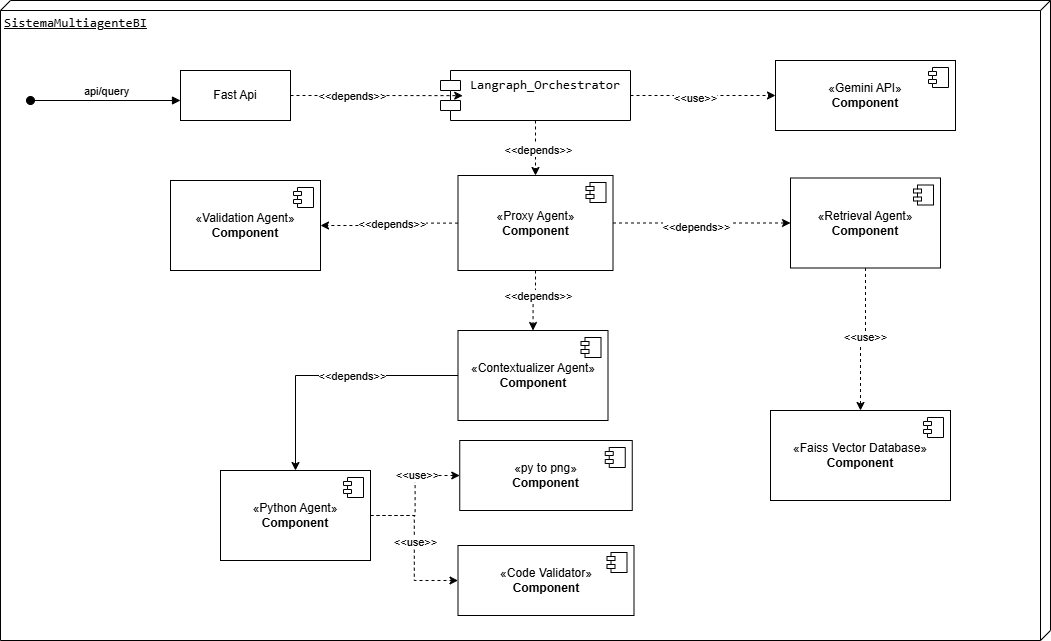
\includegraphics[width=0.7\textwidth]{images/component.png}
	\caption{Diagrama de Componentes.}
	\label{fig:Diagrama de Componente.}
\end{figure}

